\documentclass[a4paper,12pt]{article}
\usepackage{tkz-euclide}
\usepackage{gensymb}
\usepackage[utf8]{inputenc}
\usepackage{graphicx}

\title{ASSIGNMENT-4}
\author{SENANI SADHU}
\date{\today}
\begin{document}
	\maketitle
	\pagenumbering{roman}
	\section{Question:-}
	\paragraph{In $\Delta$ABC, a=6 ,$\angle$B = 60$^{\circ}$ and b-c=2. sketch the triangle.}
	\section{Solution:-}
	Given, a=6 , $\angle$B = 60$^{\circ}$ and b-c=2.\\
	Using triangle inequality property,\hspace{1cm}(To check possibility of triangle.)\\
	\begin{equation}
		b+c \textgreater  a
	\end{equation}
	but,\\
	\begin{equation}
		 b-c=2
	\end{equation}
\hspace{6cm}b=c+2\\
Therefore,\\
\hspace{4cm}2c+2\textgreater a\\
\hspace{4cm}2(c+1) \textgreater 6\\
\hspace{4cm}c \textgreater 2\\\\
Also using 2) eq, c=b-2\\
Therefore,\\
\hspace{4cm}2b-2\textgreater a\\
\hspace{4cm}2(b-1) \textgreater 6\\
\hspace{4cm}b \textgreater 4
\paragraph{Hence,$\Delta$ABC is having sides:- a=6, b \textgreater 4, c \textgreater 2.}
\subsection{Steps of Construction:-}
\begin{itemize}
	\item Draw a line BC of length a=6.
	\item  Taking B as centre  draw a line at 60$^{\circ}$ with BC.
	\item  Taking C as centre draw an arc at the distance of as b=x.
		\item Name the point where the arc and above line intersect as A.
	\item Join AB and AC.
	\item Join AB and AC.
	\item Therefore, BC=a=6, AC=b=x=5(say), AB=c=x-2=3(say)
\end{itemize}
\subsection{Figure:-}
Here assume, b=x=5 , c=x-2=3
\begin{center}
	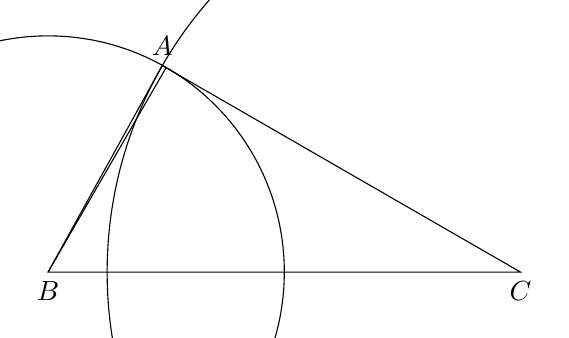
\begin{tikzpicture}[scale=1]
		\coordinate[label=below:$B$] (b) at (0,0);
		\coordinate[label=below:$C$] (c) at (6,0);
		\begin{pgfinterruptboundingbox}
			\node(Cric1) at (b) [draw, circle through=($ (b) + (0:3) $)] {};
			\node(Cric2) at (c) [draw, circle through=($ (c) + (0:5.25) $)] {};
		\end{pgfinterruptboundingbox}
		\coordinate[label=above:$A$] (a) at (intersection 2 of Cric1 and Cric2);
		\draw(b) -- (60:3cm);
		\draw(b)--(a)--(c)--cycle;
	\end{tikzpicture}
\end{center}
\newpage
\subsection{Conclusion:-}
So with given parameters as a=6, $\angle$B=60$^{\circ}$, b-c=2\\
we can have many no of triangles but these triangles are possible only when \paragraph{b \textgreater 4  and c \textgreater 2.} 
\end{document}